\chapter{大语言模型中的多步推理}\label{chap:reasoning}

\begin{learningbox}
本章将介绍语言模型如何通过{\em 多步推理（multi-step reasoning）}解决更复杂的问题。
具体而言，学完本章后，你将能够：
\begin{itemize}[leftmargin=*, nosep]
    \item 描述{\em 思维链（chain of thought）}的概念：如何利用上下文学习，引导大语言模型在回答查询时采取中间步骤，从而为更复杂的查询给出更好的答案。
    \item 说明推理方法如何大幅增强大语言模型的{\em 能力}，以及为什么智能体大语言模型要在现实世界中以符合实际的方式行动，就离不开这种能力。
    \item 编写你的第一个{\em 智能体控制框架（agentic harness）}：一个使用不同提示调用大语言模型的小型算法。智能体控制框架负责管理提示和大语言模型的回答。
    \item 解释{\em 自我反思（self-reflection）}：控制框架可以让大语言模型承担不同角色，例如{\em 评估}答案，或{\em 生成}子问题。大语言模型通过反思来改进自己的答案。
    \item 理解{\em 记忆（memory）}的作用：控制框架如何跟踪智能体的状态，以及如何利用这一状态管理提示。
    \item 运用{\em 可验证奖励强化学习（reinforcement learning with verifiable rewards，RLVR）}的概念，即将推理阶段得到的推理结果用于微调。
\end{itemize}
\end{learningbox}

\section{上下文推理}\label{sec:reasoning}
如第~\ref{chap:pipeline}~章所述，当大语言模型的参数量达到数千亿以上时，一种新的学习方式出现了。它称为{\em 上下文学习（in-context learning，ICL）}，也称{\em 提示学习（prompt-learning）} \citep{brown2020language}。这是一种重要的学习方法，本节将更详细地讨论。
随后，我们将介绍常用的基准测试，以及用于多步推理的思维链方法。

\subsection{上下文学习}
上下文学习 \citep{dong2022survey} 发生在推理阶段，而不是训练阶段。当模型被用于回答问题时，它会从大语言模型提示中提供的示例学习。
这些示例促使解码器模型访问存储在大语言模型中的相关知识。由于模型拥有丰富的知识，上下文学习只需少量示例就能找到准确结果，因此是一种所谓的{\em 少样本（few-shot）}学习方法。
少样本学习之所以可行，是因为模型规模很大，包含许多主题中丰富而多样的知识。

\paragraph{学习，而非训练}
上下文学习与微调或预训练的一个主要区别在于，上下文学习不会改变 Transformer 的参数。
由于推理阶段没有任何模型参数发生变化，它并不是一种{\em 参数训练}方法；不过，由于模型确实从给定示例中学会了如何回答，它又是一种{\em 学习}方法。
由此带来的一个缺点是遗忘：模型参数保持不变，因此，在大语言模型的两次调用之间，所有学到的信息都会丢失。要在不同调用之间共享信息，就必须将先前结果作为额外的学习示例，加入下一次调用的提示，也就是放入上下文窗口中。

\paragraph{上下文窗口}
上下文学习是如何工作的？
大语言模型中写入提示的部分，称为它的{\em 上下文窗口（context window）}。解码器模型就在这个上下文窗口内，从提示提供的示例中学习。
需要注意，模型用来学习如何回答的所有示例，都必须一起放在上下文窗口中，也就是说，它们必须能容纳在提示之内。通常，上下文窗口的大小限制在数千个词元，只能提供少量示例；因此，上下文学习能够进行的只是少样本学习。
当我们希望模型从中学习的信息量增长时，这就会成为问题，因为上下文窗口的大小通常有限。可以说，上下文学习存在长期记忆丢失的问题。

\paragraph{示例}
在上下文学习中，提示由少量用于示范的上下文片段组成，再与查询问题拼接，随后一起放入语言模型的上下文窗口 \citep{liu2023pre}。模型通过一次前向传播生成答案。例如，
如果任务是识别一条社交媒体帖子的情绪，那么在{\em 我今天没赶上公交车}之后，可以接上{\em 我感到很[\_\_\_]}，模型就可能回答{\em 难过}。
又如，在翻译任务中，我们可以在{\em 我今天没赶上公交车}之后接上
{\em 法语：[\_\_\_]}，以请求翻译。
提示包含模型能够识别的背景信息，由此选中所需的模型上下文。

\paragraph{少样本学习与机器学习的圣杯}
当语言模型包含足够的知识，能够根据提示中给出的少量示例进行泛化时，上下文学习就能发挥作用。用户在提示中提供少量相关示例，以引导大语言模型选择正确的背景知识，回答提示中的指令。
包含少量示例的上下文，称为进行少样本学习；只包含指令、完全没有示例的上下文，则称为进行零样本学习（zero-shot learning）。

上下文学习是一种让研究者十分兴奋的少样本学习形式。
在传统机器学习中，模型 $f$ 在一个数据集上训练。
要在复杂问题上达到较高准确率，数据集就必须包含大量示例。传统机器学习是一种{\em 多样本学习（many-shot learning）}，需要经过许多成本高昂的训练轮次，才能训练好模型参数。
相比之下，上下文学习成本很低，只需要少量示例，再对解码器模型进行一次前向传播即可，因为昂贵的训练已经在预训练阶段完成。少样本学习可以说是机器学习的圣杯：让模型以低成本实现泛化。

\paragraph{实践考虑与提示工程}
上下文学习还有一个实际优点，就是方便：我们可以用智能手机，在商业云端运行的大语言模型上进行上下文学习，而不必费力寻找能训练大模型的计算机。

虽然提示为使用大语言模型提供了友好的界面，但上下文学习能否成功，往往对提示的表述方式，以及所提供的不同示例相当敏感。提示学习较为脆弱，因此出现了一个称为{\em 提示工程（prompt engineering）}的新领域，帮助人类用户学习如何让大语言模型按我们的意图行事 \citep{radford2019language,wei2022emergent,giray2023prompt,sahoo2024systematic}。

在大多数大语言模型中，上下文窗口还包含隐藏的提示，即系统提示。这些提示用于指定模型的某个角色、防止使用脏话，以及在聊天机器人中提供一小段先前搜索结果的历史记录，使对话更加自然流畅。

上下文学习催生了许多后续研究。其中一个方向就是本章的主题：多步推理。推理曾经是大语言模型表现不佳的领域。例如，大语言模型连简单的数学练习都无法完成。为了更好地理解这一应用领域，我们先介绍几个推理基准测试，再讨论一种大幅提升大语言模型推理性能的上下文学习方法。

\subsection{多步推理基准测试}\label{sec:benchmarks}
人工智能的进展通过基准测试来衡量。
使用大语言模型进行多步推理的研究，始于简单的小学数学文字题。GSM8K 基准数据集就是专为研究这类简单推理而构建的 \citep{cobbe2021training}。
GSM8K 旨在提供用自然语言表述、质量高、种类多样且难度适中的问题。它包含 8500 道由人类编写的数学题及其解答。在思维链方法引入之前，语言模型很难在这个数据集上取得良好表现，详见下一节。
下面是一道典型的数学文字题：
\begin{quotation}
 \noindent {\em 问题：}Romeo 一周烤了 4 盘饼干，每盘两打。如果将这些饼干平均分给 16 个人，每人吃到多少块饼干？\\
{\em 答案：}$4\times 2\times 12/16=6$。
\end{quotation}

虽然 GSM8K 基准测试在我们看来可能很简单，事实证明它对大语言模型却很困难。该基准推出时，当时最先进的大语言模型 GPT-3-175B 的准确率仅为 15\% 左右 \citep{wei2022chain}。
其他包含类似数学文字题的基准数据集，还包括具有多种结构的 SVAMP \citep{patel2021nlp}、包含多样数学题的 ASDiv \citep{miao2021diverse}、包含代数文字题的 AQuA \citep{ling2017program}，以及 MAWPS \citep{koncel2016mawps}。

后来，其他任务的基准测试也被提出，用于评估大语言模型在其他领域的推理能力。例如，研究者开发了针对高等数学问题的基准测试（AIME \citep{codeforcesamerican}）、计算机代码理解的基准测试（Spider \citep{yu2018spider}、程序转译，即将一种计算机语言的程序翻译为另一种语言 \citep{roziere2020unsupervised}）、机器人移动的基准测试（Alfworld \citep{shridhar2020alfworld}、厨房任务 \citep{ahn2022can}）、解谜的基准测试（Game24 \citep{yao2024tree}）、创意写作的基准测试 \citep{yao2024tree}、棋盘游戏的基准测试（将杀问题 \citep{yang2024buffer}、MineCraft \citep{fan2022minedojo}），以及网页导航的基准测试（WebShop \citep{yao2022webshop}）。
其他相关基准研究还关注游戏与规划问题 \citep{ruoss2024lmact,paglieri2024balrog,wen2025thinkpatterns}。

基准测试的目标，是能够清楚地比较不同方法的性能。然而，由于实验实施方式可能不同，直接比较不同基准测试的结果有时很困难。关于大语言模型推理基准测试所面临挑战的批判性讨论，参见 \citet{kamoi2024can,shojaee2025illusion}。

\subsection{思维链提示}
2022 年前后，当时常规的大语言模型在简单数学文字题上表现不佳。值得注意的是，第~\ref{chap:scaling}~章介绍的标准方法，即通过增大模型规模来提升大语言模型性能，并没有解决这个问题 \citep{rae2021scaling}。这一问题似乎具有某种根本性，因此，研究者开始寻找不同的方法。

大语言模型采用基于 Transformer 的解码器架构。给定某个输入，它被设计为生成单个词元。大语言模型是下一个词元预测器。当我们提示这样的解码器给出答案时，它就会照着指令做：迅速给出一个答案，哪怕答案不对。但人类求解数学推理问题的方式并非如此：我们会把问题分解为一系列待求解的步骤（$4\times 2\times 12/16=6$）。因此，我们应该提示大语言模型按照一系列精心选择的中间步骤进行，逐一回答，进而得到最终答案。这就像教师教学生将复杂问题分解成较小的步骤，并要求他们在学校解题时一并给出推理步骤：{\em 不要只告诉我答案，还要告诉我你是如何{\em 得到}答案的}。儿童在学校学习解决数学问题时，会被教导将大问题分解成一系列小步骤。同样，我们也应该引导语言模型显式生成这样的中间步骤，再合并各步结果。如此一来，大语言模型的答案就应当包含中间步骤，并得出正确结果。

因此，我们的少样本提示应当包含中间推理步骤的示例，而不只是最终答案的示例。
\citet{wei2022chain} 等人研究了这个问题，并提出{\em 思维链（chain of thought，CoT）}方法。图~\ref{fig:cot}~说明了这种方法的工作方式，以及由它启发的相关方法。

要指导大语言模型生成中间步骤，可以手动编写提示，列出完成任务所需的具体推理步骤，例如计算容器中有多少个球，或馅饼被切成多少块。
\citet{wei2022chain} 尝试这一方法时，确实发现：当提示要求大语言模型在答案中将题目信息改述为中间推理步骤时，模型的表现远好于被要求直接给出单个答案时。
图~\ref{fig:cot}~展示了思维链论文中的示例。当看到较长的示例提示时，大语言模型在回答问题时也会效仿这一较长示例，即少样本 CoT。在 GSM8K 上，思维链方法使准确率从 16\% 大幅提升至 47\%。

\begin{figure}
  \begin{center}
    % 依照随附 figures/cot2.pdf 重排四面板；所有例题、算式、错误答案及代码拼写均保留。
\begingroup
\definecolor{chSixReason}{RGB}{0,145,0}
\definecolor{chSixCode}{RGB}{0,145,150}
\resizebox{\linewidth}{!}{%
\begin{tikzpicture}[x=1cm,y=1cm,
    every node/.style={font=\fontsize{8.5pt}{10.7pt}\selectfont,align=left,inner sep=0pt},
    frame/.style={draw=black!65,line width=.9pt,rounded corners=2mm},
    head/.style={draw=black!65,line width=.9pt,rounded corners=1mm,minimum width=1.8cm,minimum height=.5cm,align=center,font=\small},
    title/.style={font=\bfseries\small,align=center,text width=3.3cm},
    prompt/.style={anchor=north west,text width=3.0cm}]
\node[title] at (1.625,10.45) {少样本提示};
\node[title] at (5.175,10.45) {少样本 CoT};
\node[title] at (8.725,10.45) {零样本 CoT};
\node[title,text width=5.0cm] at (13.15,10.45) {程序辅助语言模型};
\foreach \xx/\ww in {0/3.25,3.55/3.25,7.10/3.25,10.65/5.0}{
  \draw[frame] (\xx,3.2) rectangle (\xx+\ww,9.7);
  \node[head,fill=cyan!35] at (\xx+\ww/2,9.7) {输入};
}
\node[prompt] at (.12,9.25) {问：Roger 有 5 个网球。他买了两罐球，每罐 3 个。他现在有多少个网球？\par\medskip
答：答案是 11。\par\medskip
问：Lisa 有 23 个苹果。如果她吃了 20 个，又买了 6 个，她现在有多少个苹果？};
\node[prompt] at (3.67,9.25) {问：Roger 有 5 个网球。他买了两罐球，每罐 3 个。他现在有多少个网球？\par\medskip
答：{\color{chSixReason}Rogers 最初有 5 个球。每罐 3 个，2 罐就是 6 个球。$5+6=11$。}答案是 11。\par\medskip
问：Lisa 有 23 个苹果。如果她吃了 20 个，又买了 6 个，她现在有多少个苹果？};
\node[prompt] at (7.22,9.25) {问：Lisa 有 23 个苹果。如果她吃了 20 个，又买了 6 个，她现在有多少个苹果？\par\bigskip
{\color{chSixReason}让我们一步一步地思考。}};
\node[prompt,text width=4.76cm] at (10.77,9.25) {问：Roger 有 5 个网球。他买了两罐球，每罐 3 个。他现在有多少个网球？\par\medskip
答：{\color{chSixReason}Rogers 最初有 5 个球。}\par
{\color{chSixCode}\ttfamily\fontsize{7pt}{10pt}\selectfont tennis\_balls = 5}\par
{\color{chSixReason}每罐 3 个，2 罐就是}\par
{\color{chSixCode}\ttfamily\fontsize{7pt}{10pt}\selectfont bought\_balls = 2 * 3}\par
{\color{chSixReason}个网球。}答案为\par
{\color{chSixCode}\ttfamily\fontsize{7pt}{10pt}\selectfont answer = tennis\_balls + bought\_balls}\par\medskip
问：Lisa 有 23 个苹果。如果她吃了 20 个，又买了 6 个，她现在有多少个苹果？};

\draw[frame] (0,1.3) rectangle (3.25,2.5);
\foreach \xx/\ww in {3.55/3.25,7.10/3.25,10.65/5.0}{
  \draw[frame] (\xx,-.5) rectangle (\xx+\ww,2.5);
}
\foreach \xx/\ww in {0/3.25,3.55/3.25,7.10/3.25,10.65/5.0}{
  \node[head,fill=green!40] at (\xx+\ww/2,2.5) {输出};
}
\node[prompt] at (.12,2.08) {答：答案是 27。};
\node[text=red!80!black,font=\bfseries\Large] at (2.67,1.7) {$\times$};
\node[prompt] at (3.67,2.08) {答：{\color{chSixReason}Lisa 最初有 23 个苹果。她吃了 20 个，所以还剩 $23-20=3$ 个。她又买了 6 个，因此 $3+6=9$。}答案是 9。};
\node[prompt] at (7.22,2.08) {答：{\color{chSixReason}Lisa 最初有 23 个苹果。她吃了 20 个，所以还剩 $23-20=3$ 个。她又买了 6 个，因此 $3+6=9$。}};
\node[prompt,text width=4.76cm] at (10.77,2.08) {答：{\color{chSixReason}Lisa 最初有 23 个苹果。}\par
{\color{chSixCode}\ttfamily\fontsize{7pt}{10pt}\selectfont apples = 23}\par
{\color{chSixReason}她吃了 20 个，然后又买了 6 个。}\par
{\color{chSixCode}\ttfamily\fontsize{7pt}{10pt}\selectfont eaten = 20; bought = 6}\par
{\color{chSixCode}\ttfamily\fontsize{7pt}{10pt}\selectfont anwer = apples - eaten + bought}};
\end{tikzpicture}%
}
\endgroup

    \caption{不同的思维链（CoT）提示技术 \citep{wei2022chain,kojima2022large,gao2023pal,plaat2024reasoning}。上方为提示，下方为答案。}\label{fig:cot} \label{fig:zero} \label{fig:pal}
  \end{center}
\end{figure}

只要给予提示，就能让大语言模型遵循逐步指令，这一想法令人兴奋，也开启了使用大语言模型进行多步推理的后续研究。此后，思维链成为大语言模型中的标准提示方法。

在最初的论文中，提示由研究者针对不同类型的问题手工编写。
\citet{kojima2022large} 又向前迈进了一步。
他们表明，只需添加一句与任务无关的话，即{\em 让我们一步一步地思考（Let's think step by step）}，就能显著改善许多问题上的表现。由于这句话不包含与问题有关的内容，因此属于一种零样本学习形式。
图~\ref{fig:zero}~比较了这两种方法，分别见第二列与第三列。
实验进一步表明，添加这句话后，其他推理基准测试中的性能也显著提高，包括算术推理、符号推理和逻辑推理；如果同时使用自一致性方法，详见下一节，并采用更新的 PaLM 大语言模型，在 GSM8K 上的准确率可达到 70\% \citep{wang2022self}。

思维链本身的想法受到 Scratchpad \citep{nye2021show} 的启发，也受到其他早期工作的启发，例如为算术推理生成自然语言步骤 \citep{ling2017program,cobbe2021training}，以及使用形式语言进行推理 \citep{roy2016solving,chiang2018semantically,amini2019mathqa,chen2019neural}。

\subsubsection{自我评估}
大语言模型并不完美，结果中会出现错误。
生成多个推理步骤时，错误会累积。为了避免错误失控，我们应当格外重视结果评估。
下面回顾一些减少错误累积的方法，它们或者检查模型，或者评估中间推理步骤。

当提示大语言模型进行 CoT 推理时，它会执行一系列步骤。多个步骤使模型更容易出错，也更容易受到错误累积的影响 \citep{weng2022large,xiao2023survey}。研究者已经开发出多种方法来防止错误累积。一种做法是创建一个新模型，单独评估结果。
\citet{weng2022large} 提出一种由同一个大语言模型进行评估的自动化方法，称为自我验证（self verification）。
提示要求模型将思维链推理链的结论作为求解原问题的条件，再回到原问题，比较所得答案。模型会收到自身结论的不同变体，并被要求选出与原问题相似度最高的一个。

一种流行的相关方法是自一致性（self consistency）\citep{wang2022self}。\label{selfconsistency}
自一致性是一种集成方法。集成是机器学习中的一项知名技术，通过运行多个较弱学习器来构造一个强学习器 \citep{sagi2018ensemble,breiman2001random}。
通常，大语言模型查询的答案，是从解码器网络中沿着 Logit 值最高的路径贪心提取得到的。在自一致性方法中，单条路径的贪心解码被替换为对更广泛路径样本的多数投票。
通过采样多样的推理路径、评估这些路径，并选出其中最一致的答案，自一致性实际上要求大语言模型多次执行同一个查询，再对 Transformer 模型的内部解码路径进行多数投票。自一致性之所以有效，是因为复杂推理问题通常有多条不同的推理路径可以通向正确答案。图~\ref{fig:sc}~给出了这一方法的示例。
\begin{figure}
  \begin{center}
    % 依照随附 figures/selfconsistency.pdf 中文重排；示例中的 14/26 美元错误答案故意保留。
\resizebox{\linewidth}{!}{%
\begin{tikzpicture}[x=1cm,y=1cm,
 every node/.style={font=\footnotesize,align=left,inner sep=0pt},
 frame/.style={draw=black!65,line width=1pt,rounded corners=2mm},
 head/.style={draw=black!65,line width=1pt,rounded corners=1mm,minimum height=.55cm,minimum width=2.3cm,align=center,font=\small},
 body/.style={anchor=north west,text width=3.38cm}]
\node[font=\bfseries\large,align=center] at (1.85,12.2) {少样本 CoT};
\node[font=\bfseries\large,align=center] at (10.0,12.2) {自一致性};
\draw[densely dashed,line width=1pt] (4.0,11.8) -- (4.0,12.65);
\draw[densely dashed,line width=1pt] (4.0,0) -- (4.0,6.9);
\draw[frame] (0,7.05) rectangle (16.1,11.4);
\node[head,fill=cyan!35,minimum width=5cm] at (8.05,11.4) {输入};
\node[anchor=north west,text width=15.5cm] at (.25,10.95) {问：停车场里有 3 辆车，又来了 2 辆。停车场里现在有多少辆车？\par\medskip
答：停车场里原本有 3 辆车，又来了 2 辆。现在有 $3+2=5$ 辆车。答案是 5。\par
\ldots\par
问：Janet 的鸭子每天产 16 个蛋。她每天早上吃 3 个作为早餐，并每天用 4 个给朋友烤松饼。剩下的蛋以每个 2 美元出售。她每天赚多少钱？\par
答：};
\foreach \xx in {0,4.2,8.3,12.4}{\draw[frame] (\xx,2.65) rectangle (\xx+3.7,6.4);}
\node[head,fill=green!40] at (1.85,6.4) {输出};
\node[head,fill=orange!60] at (6.05,6.4) {推理 1};
\node[head,fill=orange!60] at (10.15,6.4) {推理 2};
\node[head,fill=orange!60] at (14.25,6.4) {推理 3};
\node[body] at (.16,5.97) {这意味着她每天用掉 $3+4=7$ 个蛋。她把剩下的蛋以每个 2 美元卖出，所以每天总共卖得 $7*\$2=\$14$。\par {\color{red!85!black}答案是 14 美元。}};
\node[body] at (4.36,5.97) {她还剩 $16-3-4=9$ 个蛋。因此她每天赚 $\$2*9=\$18$。\par 答案是 18 美元。};
\node[body] at (8.46,5.97) {这意味着她每天卖出剩下的蛋，所得为 $\$2*(16-4-3)=\$26$。\par 答案是 26 美元。};
\node[body] at (12.56,5.97) {她吃了 3 个，还剩 $16-3=13$ 个。然后她烤松饼，所以剩下 $13-4=9$ 个蛋。$9$ 个蛋 $*\$2=\$18$。\par 答案是 18 美元。};
\draw[line width=.9pt,draw=black!65] (6.05,2.65) -- (10.15,1.72);
\draw[line width=.9pt,draw=black!65] (10.15,2.65) -- (10.15,1.72);
\draw[line width=.9pt,draw=black!65] (14.25,2.65) -- (10.15,1.72);
\draw[frame] (7.15,0) rectangle (13.15,1.5);
\node[head,fill=green!40] at (10.15,1.5) {输出};
\node[text=green!45!black,font=\small,align=center] at (10.15,.65) {答案是 18 美元。};
\end{tikzpicture}%
}

    \caption{自一致性，通过多数投票得到答案，改编自 \citep{wang2022self}。}\label{fig:sc}
  \end{center}
\end{figure}

研究者使用包括 GPT-3 在内的多种大语言模型，在算术推理、常识推理和符号推理上评估了自一致性。
自一致性通常能使思维链的性能再提升 10--20 个百分点。现代大语言模型经常将自一致性与思维链结合使用。

\subsubsection{生成代码以进行验证}\label{sec:selfdebug}

提高一系列推理步骤准确率的另一种方法，是从自然语言转向形式语言。形式语言的优点在于歧义比自然语言更少。Python 等计算机语言，以及数理逻辑，都是形式语言的例子。

大语言模型在根据自然语言提示生成计算机代码方面取得了相当好的成果。
\citet{chen2021evaluating} 提出了 Codex，这是一个在 GitHub 代码仓库的公开代码上训练的 GPT 模型。Codex 能够根据注释字符串等自然语言描述，生成正确的程序。
此后，使用形式语言进行推理成为一种流行方法。
许多方法用 Python 生成推理步骤，以便由编译器、调试器或解释器对代码进行评估。
人类程序员编写代码时，通常会遵循一个循环：先写一些代码，再编译并运行以查找错误，然后利用反馈改进代码。例如，自我调试（self debugging）\citep{chen2023teaching} 就采用这一方法。
它遵循相同的步骤：代码生成、代码执行和代码解释。
自我调试可以通过检查执行结果，识别自身代码中的错误，也能用自然语言解释生成的代码。

另一种方法是程序辅助语言（program aided language）\citep{gao2023pal}，它让大语言模型生成 Python，再使用解释器对结果求值。在这种方法中，问题被转化成一小段一小段的 Python 代码，再由解释器执行这些代码来解决问题。
图~\ref{fig:pal}~第四列展示了程序辅助语言方法。
当推理步骤的求值交由 Python 解释器完成时，大语言模型唯一剩下的任务，就是将自然语言问题分解为可执行的代码步骤。
\citet{gao2023pal} 提供了大量实验证据，展示神经大语言模型与符号解释器之间的协同作用。
研究者在 13 项数学、符号和算法推理任务上进行了实验，所得结果比当时规模大得多的模型更加准确；例如，程序辅助语言方法报告的准确率，在 GSM8K 上为 72\%，在 Penguins 上为 93\%。

\subsubsection{演化代码生成提示}
围绕形式语言验证的研究，催生了多项工作：无须人类反馈，自动生成针对特定问题优化、能够运行的代码。
\citet{romera2024mathematical} 提出了 FunSearch。这种方法将形式化方法与大语言模型结合，以增强数学推理与代码生成。FunSearch 采用遗传方法，维护多个候选解种群，其中的候选解就是程序，并使用由问题规范确定的函数进行评估。
评估由初始提示生成的程序之后，该方法会迭代构造新提示：选取一组采样程序，按评估分数排序并组合，再要求大语言模型生成一个新程序。
另一项工作使用演化计算方法，生成和优化演化算法 \citep{van2024llamea}。这种方法称为 LLaMEA（Large Language Model Evolutionary Algorithm），利用大语言模型设计并优化演化算法。它先用大语言模型生成初始算法结构，再通过变异与选择加以改进。
在黑箱优化基准测试（Black-Box Optimization Benchmark，BBOB）\citep{hansen2010black} 上，研究报告准确率提升了 11 个百分点。

\section{自我反思与状态}\label{sec:state}
上下文学习已经成为一种强大的新型少样本学习方法。当少样本示例指定推理步骤时，我们可以进一步增强大语言模型的能力。

本节将考察上下文学习的一些限制，以及扩展这些限制的方法。
我们先讨论状态与记忆问题：如何在大语言模型的不同调用之间传递状态，如何使用长上下文窗口，以及大语言模型是否擅长解决必须操纵状态的问题。

\subsection{大语言模型是无记忆函数}
上下文少样本学习利用大语言模型根据提示条件检索知识的能力。给定指令与示例后，Transformer 架构就在其庞大的 $(K,V)$ 参数模型中找到答案，也就是下一个词元。使用思维链提示时，大语言模型以提示中指定的少样本推理步骤为条件。

上下文学习以函数方式使用大语言模型，所有输入都通过提示提供给模型。模型 $f$ 为输入提示 $p$ 找到答案 $a$：$$f(p)\rightarrow a.$$
原则上，大语言模型不会在两次调用之间保留信息：模型参数保持不变，也没有记录历史的全局变量。如果我们希望细化请求，并将上一次调用的状态信息传递给下一次调用，就必须由用户在新提示 $p'$ 中指定所有这些状态。模型本身已经忘记了先前答案的一切。

对于聊天机器人，如果每提出一个新问题都要重复全部对话历史，那么对话就会变得累赘而不自然。在人类对话中，对方会记得刚才说过什么，无须我们显式重复其上一句话。不过，记者采访政治人物时，有时会用这种方法，试图让他们紧扣问题。
商业聊天机器人部分地通过系统提示解决这一问题：它们在用户看不到的地方，将上一次大语言模型调用的输出加入新查询的提示。然而，基本原理没有改变：大语言模型擅长根据提示，通过联想找到下一个词元的答案，却完全不擅长记住答案，以及像通用计算机编程语言那样操纵变量状态。由于没有参数发生变化，大语言模型不会在不同调用之间记住上下文状态。

\subsection{检索增强与长上下文窗口}
大语言模型的记忆问题还要更深一层。查询所需的全部信息都必须放入上下文窗口，而窗口大小有限，从根本上限制了一次查询能够传达给大语言模型的信息量。当我们要概括一本书这样的大段文本时，这一限制就会成为问题。此外，第~\ref{sec:icrl}~节将讨论上下文{\em 强化}学习方法，它们通过在上下文窗口中保存完整回合历史来工作。总之，我们需要能够向大语言模型传递更多信息的方法。

最早扩展推理阶段可用信息量的方法之一，是{\em 检索增强生成（retrieval augmentation for generative AI，RAG）}。RAG 让大语言模型调用外部数据，例如企业数据库或 Wikipedia \citep{lewis2020retrieval}。RAG 也用于减少事实性幻觉，并让模型获取具有时效性的信息，例如金融或物流数据。第~\ref{sec:rag}~章将讨论 RAG。

为了向模型传递更长文本，研究者开发了具有更长上下文窗口的大语言模型。使用标准 Transformer 架构时，计算需求随上下文窗口大小呈二次增长，因此，人们正在开发线性架构 \citep{ren2024samba}。另一种解决方案，是压缩上下文窗口中的信息，例如采用语义压缩 \citep{fei2024extending}、信息分块 \citep{wang2023augmenting,zhou2025mem1}，或递归方法 \citep{zhang2025recursive}。
为大语言模型设计新型记忆架构，是一个活跃的研究领域 \citep{yan2025general}。

\begin{figure}
    \centering
    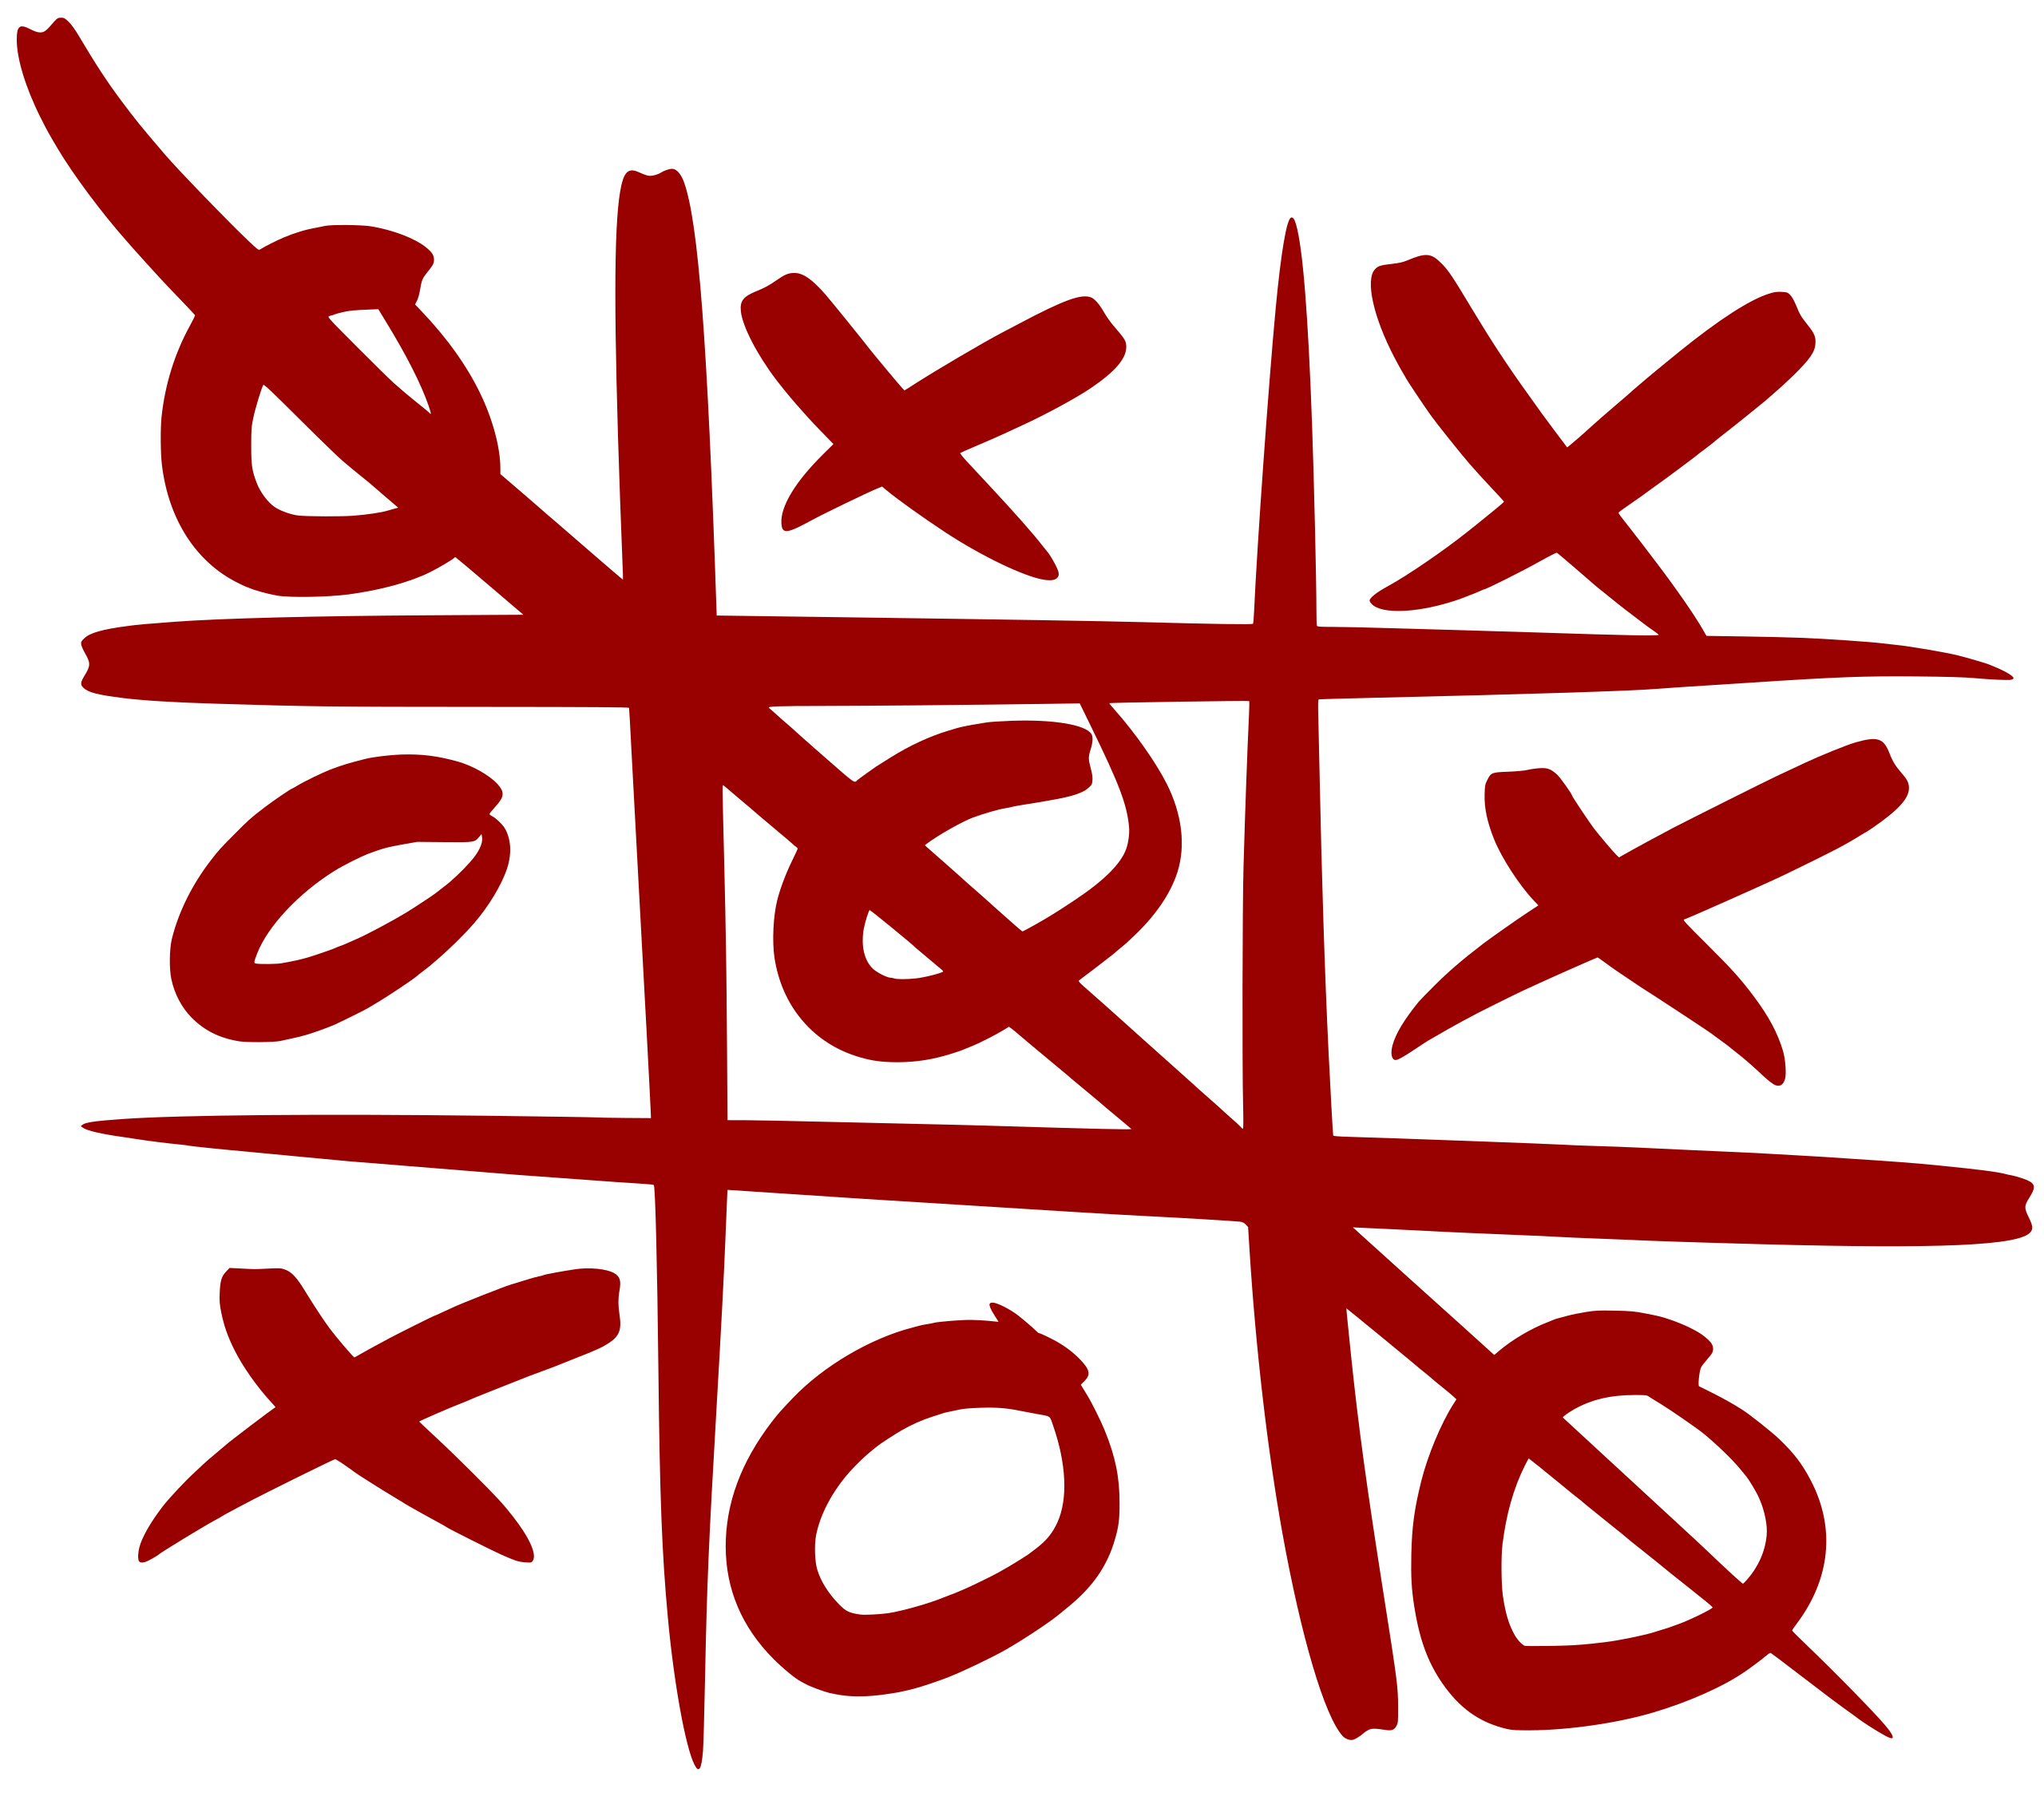
\includegraphics[width=0.35\linewidth]{figures/ttt}
    \caption{井字棋是一种简单的棋盘游戏，其中状态非常重要。}
    \label{fig:ttt}
\end{figure}

\subsection{大语言模型与有状态问题}
大语言模型在解决必须管理状态的问题时表现不佳 \citep{wong2025towards}。例如，规划问题要求准确记住当前状态；即使是图~\ref{fig:ttt}~所示的简单棋盘游戏，也有这样的要求。大语言模型往往会混淆状态，给出听起来合理的答案。这些答案对于它在训练语料中见过的棋局可能是正确的，却不适用于眼前的实际棋盘状态 \citep{paglieri2024balrog,ruoss2024lmact}。

人们已经尝试了许多方法来改进带有状态的推理，通常受到强化学习和规划算法的启发 \citep{wongstate}。
为了了解如何用大语言模型解决这些有状态问题，我们将讨论：大语言模型的无记忆特性，如何使它们受到所谓{\em 知行鸿沟（knowing-doing gap）}问题的困扰。
此外，人们还开发了其他先进方法，让大语言模型更好地处理有状态问题。第~\ref{chap:arch}~章将讨论这些进阶方法。

\paragraph{知行鸿沟}\label{sec:knowing}
除了大语言模型在不同调用{\em 之间}缺少状态之外，它在{\em 内部}执行某些任务时，还存在另一个与记忆有关的问题。

这个问题被称为{\em 知行鸿沟}。它描述了一种奇特现象：大语言模型能够生成解决问题的正确文字描述，甚至能给出正确算法，却无法正确执行该算法 \citep{paglieri2024balrog}。如果你问大语言模型如何解决某个问题，它能够迅速给出以可执行 Python 代码表示的正确算法。但随后，如果要求它真正解决这个问题，模型却不会正确遵循自己刚刚生成的算法。很多时候，它生成的算法中，变量在状态变化之间就开始出现错误 \citep{paglieri2024balrog,ruoss2024lmact}。注意，逐步忠实执行算法代码、跟踪寄存器中的数值，根本不是大语言模型中基于注意力的 Transformer 的设计目标；它们的设计目标，是通过一种联想记忆形式模拟自然语言处理 \citep{la2024code}。\footnote{还要注意，人类思维有时也存在同样的问题：我们可以轻松描述长除法算法，但在被要求计算 $12345/42$ 时，却可能犯错。计算机擅长做这件事，人类并不擅长，大语言模型也一样。}

除知行鸿沟外，还存在另一种状态管理问题。
如果提示大语言模型与自己对弈一盘棋的前几步，可能会看到棋子在两步之间神奇地出现或消失。模型没有意识到，它所走的步在某些情形下或许很好，却不适用于当前棋盘位置；它甚至还会用健谈的对话语气，为这些错误走法配上听起来合理的理由。
大语言模型难以可靠地管理变量从一个值变为另一个值的状态转换。单个数值往往会被遗忘或混淆。我们可以在提示中加入额外文字，指示模型在采取下一步之前仔细跟踪变量值 \citep{la2024code}，但这是一种繁琐且容易出错的解决方案。

通过调用外部解释器来执行大语言模型生成的算法，既可以绕过知行鸿沟，也可以避免棋子消失的问题。商业聊天机器人有时就采用这一策略。这是一个聪明而实用的解决方案，因为 Python 解释器不仅能够正确执行 Python 代码，效率也比大语言模型更高。

第~\ref{chap:arch}~章将讨论其他针对 Transformer 架构中状态与记忆问题的方法。

\subsection{用于改进提示的智能体控制框架}\label{sec:self-reflection}\label{sec:inferencetime}

除了借助外部程序执行生成的代码，人们还开发了其他方法来处理记忆和状态。本节将引入智能体方法，介绍一些小型外部算法，显式管理状态与提示。这种算法称为{\em 控制框架（harness）}。控制框架也可以用不同提示，让同一个大语言模型承担不同角色，例如状态的{\em 生成}或{\em 评估}。我们先从基于搜索算法的提示管理谈起。

当大语言模型以不同角色被调用，例如批评、评估它刚刚生成的自身表现时，可以说模型正在进行{\em 自我反思}。文献中经常用这个略带拟人色彩的术语来称呼这类方法。究竟是什么，而非“谁”，在进行自我反思：是大语言模型，还是智能体控制框架？这个问题仍有争论。

\subsubsection{基于搜索的提示优化}\label{sec:planning}
下面讨论基于搜索的推理阶段决策方法。
这些上下文学习方法超越了思维链。思维链探索的是单条推理步骤序列，每一步只有一个后继步骤；基于搜索的方法则在每一步探索多个选项，形成一棵可能性树。

当我们希望考察一棵由可能推理步骤组成的树时，就需要一种方法来跟踪状态：哪些步骤已经考察过，目前最好的答案是什么，还有哪些步骤需要进一步考察。前面已经看到，大语言模型并不十分擅长跟踪状态，而小段 Python 代码这样的常规计算机算法却很擅长。
这样的算法会将问题分解为一棵搜索树，生成多个备选步骤，并在其中向未来搜索多步，见图~\ref{fig:tot}（第~\pageref{fig:tot}~页）。算法将大语言模型作为子程序调用，通过提示要求它执行所需任务，例如动作选择和奖励评估。随后，算法可以进行回溯，尝试不同的备选步骤。这个控制算法位于大语言模型之外，包裹着模型，负责跟踪状态、管理提示，使其与外界隔离，也保护外界免受状态管理混乱的大语言模型影响。这个控制算法称为{\em 控制框架}。

我们从深度优先搜索与广度优先搜索开始讨论控制策略 \citep{cormen2022introduction}。
\label{sec:buffer}
思维树（tree of thoughts，ToT）\citep{yao2024tree} 使用广度优先或深度优先搜索，动态沿着不同推理步骤展开。\footnote{思维树是一种流行的方法。Huggingface 链接见：\url{https://huggingface.co/blog/sadhaklal/tree-of-thoughts}。}
思维树中的生成部分，即红色部分，以及评估部分，即绿色部分，都是通过提示大语言模型完成的，见图~\ref{fig:totcode}。
\begin{figure}
  \begin{center}
    % 依照 figures/totcode.png 中文重排伪代码。函数、集合、参数和控制语句不变；红/绿箭头对应 G/V 提示。
\usetikzlibrary{shapes.geometric}
\resizebox{\linewidth}{!}{%
\begin{tikzpicture}[x=1cm,y=1cm,
 every node/.style={font=\fontsize{8.5pt}{11pt}\selectfont,align=left,inner sep=2pt},
 code/.style={anchor=west},
 role/.style={font=\fontsize{8.5pt}{11pt}\selectfont,align=center},
 gcall/.style={draw=red!85!black,ellipse,line width=1pt,inner sep=4pt},
 vcall/.style={draw=green!55!black,ellipse,line width=1pt,inner sep=4pt},
 gflow/.style={-{Stealth[length=2.5mm,width=2mm]},draw=red!85!black,line width=1pt},
 vflow/.style={-{Stealth[length=2.5mm,width=2mm]},draw=green!55!black,line width=1pt}]
\draw[line width=.8pt] (0,9.95) -- (8.15,9.95);
\draw[line width=.5pt] (0,9.15) -- (8.15,9.15);
\node[code,font=\fontsize{9pt}{11pt}\selectfont] at (.1,9.55) {\textbf{算法 1}\quad $\mathrm{ToT\!\! -\! BFS}(x,p_\theta,G,k,V,T,b)$};
\node[anchor=north west,text width=7.7cm] at (.1,8.95) {\textbf{要求：}输入 $x$，语言模型 $p_\theta$，规模上限 $k$，步数上限 $T$，广度上限 $b$。};
\node[role,text=green!45!black] (bvrole) at (2.35,7.65) {状态评估器 $V()$};
\node[role,text=red!80!black] (bgrole) at (6.1,7.65) {思维生成器 $G()$};
\node[code] at (.65,6.8) {$S_0\leftarrow\{x\}$};
\node[code] at (.65,6.2) {\textbf{for} $t=1,\ldots,T$ \textbf{do}};
\node[code] at (1.0,5.5) {$S'_t\leftarrow\{[s,z_t]\mid s\in S_{t-1},$};
\node[code] at (1.45,4.9) {$z_t\in$};
\node[gcall] (bg) at (4.45,4.9) {$G(p_\theta,s,k)$};
\node[code] at (6.18,4.9) {$\}$};
\node[code] at (1.0,4.1) {$V_t\leftarrow$};
\node[vcall] (bv) at (3.65,4.1) {$V(p_\theta,S'_t)$};
\node[code] at (1.0,3.2) {$S_t\leftarrow\argmax_{S\subset S'_t,|S|=b}\sum_{s\in S}V_t(s)$};
\node[code] at (.65,2.4) {\textbf{end for}};
\node[code] at (.65,1.55) {\textbf{return} $G(p_\theta,\argmax_{s\in S_T}V_T(s),1)$};
\draw[gflow] (bg.north) to[out=90,in=180] (7.7,5.95) -- (7.7,7.65) -- (bgrole.east);
\draw[vflow] (bv.north) -- (3.65,4.6) -- (.2,4.6) -- (.2,7.65) -- (bvrole.west);
\draw[line width=.5pt] (0,.8) -- (8.15,.8);

\begin{scope}[xshift=8.65cm]
\draw[line width=.8pt] (0,9.95) -- (8.15,9.95);
\draw[line width=.5pt] (0,9.15) -- (8.15,9.15);
\node[code,font=\fontsize{9pt}{11pt}\selectfont] at (.1,9.55) {\textbf{算法 2}\quad $\mathrm{ToT\!\! -\! DFS}(s,t,p_\theta,G,k,V,T,v_{th})$};
\node[anchor=north west,text width=7.7cm] at (.1,8.95) {\textbf{要求：}当前状态 $s$，步骤 $t$，语言模型 $p_\theta$，规模上限 $k$，步数上限 $T$，阈值 $v_{th}$。};
\node[role,text=green!45!black] (dvrole) at (2.35,7.65) {状态评估器 $V()$};
\node[role,text=red!80!black] (dgrole) at (6.1,7.65) {思维生成器 $G()$};
\node[code] at (.65,6.8) {\textbf{if} $t>T$ \textbf{then}};
\node[code] at (1.1,6.25) {记录输出 $G(p_\theta,s,1)$};
\node[code] at (.65,5.7) {\textbf{end if}};
\node[code] at (.65,5.0) {\textbf{for} $s'\in$};
\node[gcall] (dg) at (4.1,5.0) {$G(p_\theta,s,k)$};
\node[code] at (5.75,5.0) {\textbf{do}};
\node[code,font=\scriptsize] at (5.55,4.52) {$\triangleright$ 已排序候选};
\node[code] at (1.0,4.0) {\textbf{if}};
\node[vcall] (dv) at (3.5,4.0) {$V(p_\theta,\{s'\},x)$};
\node[code] at (5.13,4.0) {$>v_{thres}$ \textbf{then}};
\node[code,font=\scriptsize] at (5.55,3.45) {$\triangleright$ 剪枝};
\node[code] at (1.5,2.85) {$\mathrm{DFS}(s',t+1)$};
\node[code] at (1.0,2.2) {\textbf{end if}};
\node[code] at (.65,1.55) {\textbf{end for}};
\draw[gflow] (dg.north) to[out=90,in=180] (7.75,6.0) -- (7.75,7.65) -- (dgrole.east);
\draw[vflow] (dv.north) -- (3.5,4.5) -- (.2,4.5) -- (.2,7.65) -- (dvrole.west);
\draw[line width=.5pt] (0,.8) -- (8.15,.8);
\end{scope}
\end{tikzpicture}%
}

    \caption{思维树。左侧为广度优先搜索，右侧为深度优先搜索。箭头表示大语言模型提示，改编自 \citep{yao2024tree}。} \label{fig:totcode}
  \end{center}
\end{figure}
两个大语言模型提示与外部控制结合起来，就能系统地探索推理步骤空间，进行前瞻与回溯。

\begin{figure}
  \begin{center}
    % 依照 figures/tot-ex.png 重绘。原例的所有数字、运算符、剩余数字和评价均逐项保留。
\resizebox{\linewidth}{!}{%
\begin{tikzpicture}[x=1cm,y=1cm,
 every node/.style={font=\footnotesize,align=left,inner sep=2pt},
 tree/.style={font=\fontsize{8.5pt}{10pt}\selectfont,align=center,inner sep=1pt},
 leftnums/.style={font=\scriptsize,align=center,inner sep=1pt},
 edge/.style={-{Stealth[length=1.6mm,width=1.2mm]},draw=black!60,line width=.6pt},
 card/.style={draw=black!60,rounded corners=1mm,line width=.7pt},
 header/.style={draw=black!60,rounded corners=.8mm,line width=.7pt,font=\bfseries\small,minimum height=.55cm},
 body/.style={anchor=north west,text width=3.6cm},
 call/.style={draw=black!60,rounded corners=1.5mm,font=\bfseries\Large,minimum width=1.0cm,minimum height=1.1cm},
 link/.style={-{Stealth[length=2.5mm,width=2mm]},draw=black!60,line width=1.0pt}]
\node[tree,font=\bfseries\small] at (2.3,7.65) {输入：4 9 10 13};
\draw[dashed,draw=black!60,line width=.9pt] (.2,6.6) rectangle (4.4,7.25);
\foreach \xx in {.65,2.3,3.95}{\draw[edge] (2.3,7.2) -- (\xx,6.6);}
\node[tree] at (.55,6.2) {$\cdots$};
\node[tree,text=green!55!black] (a) at (2.3,6.2) {$10-4=6$};
\node[leftnums,text=green!55!black] at (2.3,5.85) {余：6 9 13};
\node[tree,text=red!85!black] at (3.95,6.2) {$4+9=13$};
\node[leftnums,text=red!85!black] at (3.95,5.85) {余：10 13 13};
\draw[dashed,draw=orange!85!black,line width=1pt] (3.13,5.45) rectangle (4.77,6.57);
\foreach \xx in {.65,2.3,3.95}{\draw[edge] (2.3,5.35) -- (\xx,4.98);}
\node[tree,text=red!85!black] at (.65,4.65) {$13-6=7$};
\node[leftnums,text=red!85!black] at (.65,4.3) {余：7 9};
\node[tree,text=green!55!black] at (2.3,4.65) {$13-9=4$};
\node[leftnums,text=green!55!black] at (2.3,4.3) {余：4 6};
\node[tree] at (3.95,4.65) {$\cdots$};
\foreach \xx in {.65,2.3,3.95}{\draw[edge] (2.3,3.85) -- (\xx,3.43);}
\node[tree,text=red!85!black] at (.65,3.1) {$4+6=10$};
\node[leftnums,text=red!85!black] at (.65,2.75) {余：10};
\node[tree,text=green!55!black] at (2.3,3.1) {$4*6=24$};
\node[leftnums,text=green!55!black] at (2.3,2.75) {余：24};
\node[tree] at (3.95,3.1) {$\cdots$};

\draw[card] (5.1,4.9) rectangle (9.0,7.5);
\node[header,fill=black!7,minimum width=3.9cm] at (7.05,7.2) {(a) 提议提示};
\node[body] at (5.23,6.68) {{\color{black!45}\emph{（一个示例）}}\par
输入：\colorbox{black!8}{4 9 10 13}\par
可能的下一步：};
\node[call] (lm1) at (10.2,6.0) {LM};
\draw[link] (9.0,6.0) -- (lm1.west);
\draw[link] (lm1.east) -- (11.5,6.0);
\draw[card] (11.5,4.9) rectangle (17.0,7.5);
\node[header,fill=black!7,minimum width=5.5cm] at (14.25,7.2) {思维生成};
\node[body,text width=5.2cm] at (11.63,6.68) {$4+9=13$（剩余：10 13 13）\par
$10-4=6$（剩余：6 9 13）\par
{\color{black!45}\emph{（\ldots 更多行\ldots）}}};

\draw[card] (5.1,.6) rectangle (9.0,4.25);
\node[header,fill=orange!15,text=orange!65!black,minimum width=3.9cm] at (7.05,3.95) {(b) 价值提示};
\node[body] at (5.23,3.43) {评估给定数字能否得到 24（确定／可能／不可能）\par
10 14：$10+14=24$。确定\par
{\color{black!45}\emph{（更多示例）}}\par
\colorbox{red!12}{10 13 13}};
\node[call] (lm2) at (10.2,2.35) {LM};
\draw[link] (9.0,2.35) -- (lm2.west);
\draw[link] (lm2.east) -- (11.5,2.35);
\draw[card] (11.5,.6) rectangle (17.0,4.25);
\node[header,fill=orange!15,text=orange!65!black,minimum width=5.5cm] at (14.25,3.95) {思维评估};
\node[body,text width=5.2cm] at (11.63,3.43) {$(13-10)*13=3*13=39$\par
$10+13+13=36$。用这些大数无法得到 24。\colorbox{red!12}{不可能}};
\draw[-{Stealth[length=3mm,width=3mm]},draw=black!60,line width=2.2pt] (4.5,6.93) -- (5.0,6.93);
\draw[-{Stealth[length=3mm,width=3mm]},draw=orange!80!black,line width=2.0pt] (4.6,5.35) -- (5.0,4.3);
\end{tikzpicture}%
}

    \caption{24 点游戏的思维树提示示例 \citep{yao2024tree}。} \label{fig:tot-ex}
  \end{center}
\end{figure}

思维树（ToT）已经用于 24 点游戏这类基于规划的谜题。游戏给出 4 个数，任务是在这些数之间使用算术运算符 $( + - * / )$，得到 24。例如，对于数字 $4$ $9$ $10$ $13$，一个解是 $(10-4)*(13-9)=24$。思维树首先使用{\em 提议（propose）}提示生成一个局面：\verb|Input 4 9 10 13; Possible next steps:|，模型据此生成可能的下一步思考。随后，模型使用包含思维链示例的评估提示，对这些思考进行评估。图~\ref{fig:tot-ex}~展示了原论文中一个可能的提示序列。

作者在 24 点游戏、创意写作与迷你填字游戏上，将该方法与结合自一致性的传统线性思维链进行比较，在一项 24 点游戏任务上达到了 74\% 的准确率。其他任务则采用定性评估。
图~\ref{fig:tot}~说明了不同的推理结构。\footnote{另一种名称相似的方法是思维图（graph of thoughts）\citep{besta2024graph}。思维图允许更一般的推理图结构，提供一个形式化框架，其中不同要素可以手动指定。}

\begin{figure}
  \begin{center}
    % 依照 figures/cot-tot.png 重绘，保留四面板、全部状态节点和原有连线。
\begingroup
\definecolor{chSixLeaf}{RGB}{142,196,61}
\definecolor{chSixFail}{RGB}{190,35,43}
\resizebox{\linewidth}{!}{%
\begin{tikzpicture}[x=1cm,y=1cm,
 every node/.style={font=\small,align=center,inner sep=3pt},
 io/.style={draw=black!65,line width=1.2pt,rounded corners=1.5mm,minimum width=2.1cm,minimum height=.65cm},
 state/.style={draw=black!65,line width=1.1pt,rounded corners=1.3mm,minimum width=.95cm,minimum height=.55cm,fill=black!25},
 flow/.style={-{Stealth[length=2mm,width=1.6mm]},draw=black!65,line width=1.1pt},
 panel/.style={font=\small,align=center,text width=3cm}]
\foreach \xx/\id in {1.3/a,4.1/b,8.7/c,14.1/d}{
 \node[io,fill=cyan!35] (in\id) at (\xx,7.3) {输入};
 \node[io,fill=green!40] (out\id) at (\xx,.4) {输出};
}
\draw[flow] (ina.south) -- (outa.north);
\node[state] (b1) at (4.1,5.6) {};
\node[state] (b2) at (4.1,3.4) {};
\draw[flow] (inb.south) -- (b1.north);
\draw[draw=black!65,line width=1.1pt] (b1.south) -- (4.1,4.85);
\node at (4.1,4.55) {$\cdots$};
\draw[flow] (4.1,4.23) -- (b2.north);
\draw[flow] (b2.south) -- (outb.north);

\foreach \xx/\i/\cc in {7.0/1/chSixLeaf,8.7/2/chSixLeaf,10.4/3/chSixFail}{
 \node[state] (c\i a) at (\xx,5.7) {};
 \node[state] (c\i b) at (\xx,4.0) {};
 \node[state,fill=\cc] (c\i c) at (\xx,2.3) {};
 \draw[flow] (inc.south) -- (c\i a.north);
 \node at (\xx,4.95) {$\cdots$};
 \draw[flow] (\xx,4.65) -- (c\i b.north);
 \draw[flow] (c\i b.south) -- (c\i c.north);
}
\draw[decorate,decoration={brace,mirror,amplitude=4pt},line width=.8pt] (6.48,1.87) -- (9.22,1.87);
\node[font=\footnotesize] at (7.85,1.4) {多数投票};

\node[state,fill=green!20!gray!35] (d11) at (12.7,5.7) {};
\node[state,fill=green!35!gray!25] (d12) at (14.1,5.7) {};
\node[state,fill=red!30!gray!40] (d13) at (15.5,5.7) {};
\foreach \i in {1,2,3}{\draw[flow] (ind.south) -- (d1\i.north);}
\node[state,fill=green!20!gray!35] (d21) at (12.1,4.0) {};
\node[state,fill=red!30!gray!40] (d22) at (13.4,4.0) {};
\node[state,fill=green!50!gray!20] (d23) at (14.8,4.0) {};
\node[state,fill=red!30!gray!40] (d24) at (16.1,4.0) {};
\draw[flow] (d11.south) -- (d21.north);
\foreach \i in {2,3,4}{\draw[flow] (d12.south) -- (d2\i.north);}
\foreach \xx/\i/\cc in {12.1/1/chSixFail,13.4/2/chSixFail,14.8/3/chSixLeaf,16.1/4/chSixFail}{
 \node[state,fill=\cc] (d3\i) at (\xx,2.3) {};
}
\draw[flow] (d21.south) -- (d31.north);
\draw[flow] (d21.south) -- (d32.north);
\draw[flow] (d23.south) -- (d33.north);
\draw[flow] (d23.south) -- (d34.north);

\node[panel,text width=2.5cm] at (1.3,-.65) {(a) 输入—输出\\提示（IO）};
\node[panel,text width=2.5cm] at (4.1,-.65) {(b) 思维链\\提示（CoT）};
\node[panel,text width=4.8cm] at (8.7,-.65) {(c) 结合 CoT 的自一致性\\（CoT-SC）};
\node[panel,text width=4.8cm] at (14.1,-.65) {(d) 思维树\\（ToT）};
\end{tikzpicture}%
}
\endgroup

    \caption{思维链（b）、自一致性（c）与思维树（d）的推理结构。} \label{fig:tot} \label{fig:bot}
  \end{center}
\end{figure}

思维树是一种简洁优雅的方法，在大语言模型之上加入了两种极为简单的搜索结构。提示序列容易理解，也容易发现和纠正错误。

思维树的两种搜索方法都遵循固定的扩展策略。
接下来，我们将讨论更先进的基于学习的方法。它们可能表现更好，但代价是更高的算法复杂度。

\subsubsection{自我反思}\label{sec:reflective}\label{sec:selfreflection}
人们已经设计了许多让大语言模型承担不止一种角色的方法。这类方法通常称为自我反思方法。大语言模型不仅用于评估提示，还用于生成新的推理步骤，并且经常进一步改进这些步骤。

自我反思领域还很年轻，新方法不断涌现。我们将介绍其中四种：Self Refine、ReAct、Reflexion 和思维缓冲。这些方法以不同方式使用大语言模型，借鉴强化学习的方案，让模型自我改进。

\paragraph{Self Refine} 第一种方法是 Self Refine \citep{madaan2023self}，旨在通过反馈改进答案。
大语言模型先生成初始输出，再为自己的答案提供反馈，用自身迭代地改进自身。因此，大语言模型被用于改进自己的答案，见图~\ref{fig:refine}。
 \begin{figure}
   \begin{center}
     % 依照 figures/selfref.png 重绘，保留输入、模型、反馈、改进与 0/1/2 循环编号。
\resizebox{.9\linewidth}{!}{%
\begin{tikzpicture}[x=1cm,y=1cm,
 every node/.style={font=\normalsize,align=center,inner sep=4pt},
 box/.style={draw=black,line width=1pt,minimum height=.85cm},
 flow/.style={-{Stealth[length=3mm,width=2.4mm]},line width=1.6pt},
 stage/.style={draw=black,circle,fill=white,font=\small,inner sep=2pt}]
\draw[line width=.9pt] (0,0) rectangle (14.4,6.0);
\node[box,fill=blue!8,minimum width=2.4cm] (input) at (7.2,5.15) {输入};
\node[box,fill=violet!20,minimum width=3.0cm,minimum height=2.2cm] (model) at (7.2,2.9) {模型 $\mathcal{M}$};
\node[box,fill=red!25,minimum width=3.8cm] (feedback) at (2.3,2.9) {反馈};
\node[box,fill=orange!20,minimum width=3.8cm] (refine) at (12.1,2.9) {改进};
\draw[flow] (input.south) -- node[stage,left=2pt] {$0$} (model.north);
\draw[flow] (model.north west) to[out=155,in=90] (feedback.north);
\draw[flow] (feedback.south) to[out=-90,in=210] node[stage,pos=.45] {$1$} (model.south west);
\draw[flow] (model.north east) to[out=25,in=90] (refine.north);
\draw[flow] (refine.south) to[out=-90,in=-30] node[stage,pos=.45] {$2$} (model.south east);
\node[fill=black!7,rounded corners=1mm,text width=6.4cm,font=\small,minimum height=.55cm] at (3.6,.45) {用 $\mathcal{M}$ 对自身输出给出反馈};
\node[fill=black!7,rounded corners=1mm,text width=6.4cm,font=\small,minimum height=.55cm] at (10.8,.45) {根据反馈，用 $\mathcal{M}$ 改进先前输出};
\end{tikzpicture}%
}

     \caption{Self Refine 架构 \citep{madaan2023self}。}\label{fig:refine}
  \end{center}
\end{figure}
Self Refine 以三种方式提示大语言模型：(1) 初始生成；(2) 反馈；(3) 改进，沿着一条贪心推理链推进。据报告，在对话回答生成、代码优化和受约束生成等基准测试上，Self Refine 显著优于常规思维链。不过，这种方法确实遵循一条线性、贪心的推理链，在每个状态只尝试一个后继，并不像 ToT 那样探索一棵树。

\paragraph{ReAct}
将贪心方法推广后，我们可以使用大语言模型考察每个状态下的多个选项。
ReAct 是一种值得关注的结合强化学习与大语言模型的方法 \citep{yao2022react}。\footnote{\url{https://github.com/ysymyth/ReAct}}
ReAct 将思维链提示学习作为强化学习框架的一部分，同时使用外部知识源 Wikipedia 与微调，以减少错误、进行锚定并降低幻觉。该框架允许使用手工编写的提示。
在 Alfworld 与 WebShop 两个交互式决策基准测试上，ReAct 分别以 34\% 和 10\% 的绝对成功率提升，胜过模仿学习与强化学习方法。

\paragraph{Reflexion}
ReAct 的工作后来得到进一步发展。
Reflexion \citep{shinn2024reflexion} 受到人类做法的启发，构建能够通过反思失败来学习、并改善结果的人工智能智能体。\footnote{\url{https://github.com/noahshinn/reflexion}}
Reflexion 为大语言模型使用三种提示：行动者、评估者与反思者。
Reflexion 控制框架在大语言模型的不同调用之间加入显式记忆。它用短期记忆生成轨迹，用长期记忆保存经验信息。通过在外部算法中使用记忆，这种方法处理了常规大语言模型的状态管理问题。Reflexion 的工作过程如下：(1) 行动者模型生成文本与动作；(2) 评估者模型为行动者产生的输出评分；(3) 自我反思模型生成文字形式的强化线索，帮助行动者自我改进，见图~\ref{fig:reflexion2}。
行动者可以采用思维链与 ReAct。Reflexion 已在决策、推理和编程任务上进行评估，据报告可提升 10--20 个百分点 \citep{shinn2024reflexion}。
\begin{figure}
  \begin{center}
    % 依照 figures/reflexion3.png 重绘，全部外部/内部反馈、轨迹、经验和动作连线对应原图。
\resizebox{.9\linewidth}{!}{%
\begin{tikzpicture}[x=1cm,y=1cm,
 every node/.style={font=\normalsize,align=center,inner sep=4pt},
 lm/.style={draw=black!60,fill=cyan!8!gray!15,rounded corners=1.5mm,line width=.8pt,minimum width=4.5cm,minimum height=.85cm},
 memory/.style={draw=black!60,fill=yellow!15,line width=.8pt,minimum width=4.4cm,minimum height=1.2cm},
 flow/.style={-{Stealth[length=2.5mm,width=1.8mm]},draw=black!60,line width=.9pt},
 label/.style={font=\small,fill=black!2,inner sep=2pt}]
\filldraw[draw=black!60,fill=black!2,line width=.8pt] (.6,2.5) rectangle (12.8,10.2);
\node[font=\bfseries\Large] at (6.7,9.55) {智能体};
\node[lm] (reflect) at (7.0,8.2) {自我反思（LM）};
\node[lm] (eval) at (3.7,6.25) {评估者（LM）};
\node[memory] (traj) at (3.7,4.0) {轨迹\\（短期记忆）};
\node[memory] (experience) at (9.7,6.0) {经验\\（长期记忆）};
\node[lm] (actor) at (9.7,4.0) {行动者（LM）};
\node[draw=black!60,fill=black!7,line width=.8pt,minimum width=4.5cm,minimum height=.9cm,font=\bfseries\large] (env) at (6.4,.7) {环境};

\draw[flow] (traj.north) -- (eval.south);
\draw[flow] (traj.east) -- (actor.west);
\draw[flow] (experience.south) -- (actor.north);
\draw[flow] (reflect.east) -- (10.3,8.2) -- (10.3,6.6);
\node[label] at (11.25,7.35) {反思文本};
\draw[draw=black!60,line width=.9pt] (eval.north) -- (3.7,8.2);
\node[label] at (2.65,7.35) {内部\\反馈};
\draw[flow] (env.west) -- (0,.7) -- (0,8.2) -- (reflect.west);
\node[label] at (2.65,8.65) {外部反馈};
\draw[flow] (0,4.0) -- (traj.west);
\node[font=\normalsize,fill=white,inner sep=4pt] at (2.1,.7) {观测／奖励};
\draw[flow] (actor.east) -- (13.3,4.0) -- (13.3,.7) -- (env.east);
\node[font=\normalsize,fill=white,inner sep=4pt] at (10.8,.7) {动作};
\end{tikzpicture}%
}

    \caption{Reflexion 架构 \citep{shinn2024reflexion}，与强化学习的智能体／环境结构十分相似。}\label{fig:reflexion2}
  \end{center}
\end{figure}

\paragraph{思维缓冲}
另一种方法是思维缓冲（buffer of thoughts）\citep{yang2024buffer}，它向元推理（metareasoning）\citep{gao2024meta} 又迈进了一步。这种方法引入一个元缓冲区，保存高层{\em 思维模板（thought-template）}。思维模板来自多种任务。思维缓冲使用一个问题蒸馏器，将从不同问题中蒸馏出的高层思维存入元缓冲区，并主动管理其容量。图~\ref{fig:bot2}~将思维缓冲与思维链、思维树等方法进行比较。在 24 点游戏与将杀等谜题上，思维缓冲优于其他方法，提升幅度分别为 11\% 和 51\%。
思维模板与元认知（metacognition），即思考如何思考，有关 \citep{didolkar2024metacognitive}。
 \begin{figure}
   \begin{center}
     % 依照 figures/bot.png 重绘三种结构和元缓冲区的三条关系，不改变原图的比较方向。
\usetikzlibrary{shapes.geometric}
\begingroup
\definecolor{chSixBufferBlue}{RGB}{148,190,224}
\resizebox{\linewidth}{!}{%
\begin{tikzpicture}[x=1cm,y=1cm,
 every node/.style={font=\small,align=center,inner sep=3pt},
 llm/.style={fill=black!15,rounded corners=1.5mm,minimum width=1.8cm,minimum height=.8cm},
 think/.style={draw=blue!40,fill=yellow!18,rounded corners=1.5mm,minimum width=2.0cm,minimum height=.8cm},
 bot/.style={fill=chSixBufferBlue,rounded corners=1.5mm,minimum width=2.0cm,minimum height=.8cm},
 output/.style={ellipse,fill=black!15,minimum width=1.8cm,minimum height=.8cm},
 flow/.style={-{Stealth[length=2mm,width=1.5mm]},line width=.6pt},
 memoryflow/.style={-{Stealth[length=2.5mm,width=2mm]},draw=chSixBufferBlue,line width=1.4pt},
 caption/.style={font=\small,align=center,text width=3.4cm},
 effect/.style={font=\bfseries\small,align=center}]
\foreach \yy/\i in {10.4/1,7.4/2,4.5/3}{
 \node[anchor=east] at (1.6,\yy) {输入查询};
 \node[font=\large] at (1.87,\yy) {$+$};
 \node[llm] (llm\i) at (3.1,\yy) {LLM};
 \node[output] (out\i) at (14.0,\yy) {输出};
}

\node[think] (reason1) at (10.1,10.4) {推理};
\draw[flow] (llm1.east) -- (reason1.west);
\draw[flow] (reason1.east) -- (out1.west);
\node[font=\bfseries\small] at (6.55,10.78) {单次查询};
\node[caption,text width=4.8cm] at (6.55,9.83) {针对具体任务的手工提示\\（如 CoT、少样本提示）};
\node[effect] at (14.0,9.55) {准确率};
\draw[-{Stealth[length=2.5mm]},line width=1.5pt] (14.95,9.95) -- (14.95,9.2);

\node[think] (expand) at (6.8,7.4) {思维扩展};
\node[think] (reason2) at (10.1,7.4) {推理};
\draw[flow] (llm2.east) -- (expand.west);
\draw[flow] (expand.east) -- (reason2.west);
\draw[flow] (reason2.east) -- (out2.west);
\node[font=\bfseries\small] at (4.95,7.8) {多次查询};
\node[caption,text width=3cm] at (4.9,6.7) {预定义查询结构\\（如 ToT、GoT）};
\draw[-{Stealth[length=3mm,width=2.4mm]},draw=blue!70!black,double=yellow!55,double distance=1.0pt,line width=.5pt] (reason2.north) to[out=105,in=75] (expand.north);
\draw[-{Stealth[length=3mm,width=2.4mm]},draw=blue!70!black,double=yellow!55,double distance=1.0pt,line width=.5pt] (expand.south) to[out=-75,in=-105] (reason2.south);
\node[font=\bfseries\small,fill=white,inner sep=2pt] at (8.45,8.95) {$N$ 跳迭代};
\node[effect] at (14.0,6.55) {效率};
\draw[-{Stealth[length=2.5mm]},line width=1.5pt] (14.95,6.95) -- (14.95,6.2);

\draw[dashed,line width=.8pt] (0,5.6) -- (15.7,5.6);
\node[bot] (distiller) at (6.45,4.5) {问题蒸馏器};
\node[bot,font=\bfseries\small] (instance) at (10.1,4.5) {实例化推理};
\node[bot,font=\bfseries\small,text=red!80!black,minimum width=2.4cm] (meta) at (10.1,1.0) {元缓冲区};
\draw[flow] (llm3.east) -- (distiller.west);
\draw[memoryflow] (distiller.east) -- (instance.west);
\draw[memoryflow] (instance.east) -- (out3.west);
\draw[memoryflow] (6.2,4.1) -- (9.0,.8);
\draw[memoryflow] (8.9,1.25) -- (6.8,4.1);
\draw[memoryflow,dashed] (14.0,4.1) -- (11.3,1.1);
\node[caption,text width=1.8cm,fill=white,inner sep=1pt] at (7.1,1.9) {高层思维};
\node[caption,text width=1.8cm,fill=white,inner sep=1pt] at (8.75,3.15) {思维检索};
\node[caption,text width=1.9cm,fill=white,inner sep=1pt] at (11.65,2.85) {思维蒸馏\\与更新};
\node[effect] at (14.0,2.95) {准确率\\与\\效率};
\draw[-{Stealth[length=2.5mm]},draw=red!80!black,line width=1.5pt] (14.95,2.3) -- (14.95,3.6);
\node[font=\bfseries\large] at (2.9,.55) {思维缓冲（BoT）};

% 与原图一致的两张愁脸和一张笑脸。
\foreach \yy in {8.9,5.95}{
 \fill[black] (14.0,\yy) circle (.23);
 \fill[white] (13.92,\yy+.07) circle (.026);
 \fill[white] (14.08,\yy+.07) circle (.026);
 \draw[white,line width=.7pt] (13.89,\yy-.10) .. controls (14.0,\yy+.05) .. (14.11,\yy-.10);
}
\fill[black] (14.0,1.8) circle (.23);
\fill[white] (13.92,1.87) circle (.026);
\fill[white] (14.08,1.87) circle (.026);
\draw[white,line width=.7pt] (13.89,1.79) .. controls (14.0,1.59) .. (14.11,1.79);
\end{tikzpicture}%
}
\endgroup

     \caption{思维缓冲 \citep{yang2024buffer}。}\label{fig:bot2}
   \end{center}
 \end{figure}

\paragraph{批评与提示敏感性}
自我反思概念也存在陷阱，并受到批评。首先，要求模型改进自身结果这一基本想法，会引出一个问题：为什么模型一开始没有给出更好的答案？其次，\citet{huang2023large,shojaee2025illusion} 的研究发现，一些研究存在方法论问题，例如使用泄露答案的数据标签、第二次改进提示无意中透露了比初始提示更多的信息，以及使用同一个大语言模型同时充当智能体与环境。在一项可复现性研究中，性能没有超过结合自一致性的思维链 \citep{huang2023large}。大语言模型对提示中问题的表述方式很敏感。自我反思仍是一个年轻而活跃的研究领域，前提设想很有吸引力，但还存在许多开放问题。

前面介绍的方法可能需要多次调用大语言模型，因而成本很高，速度也很慢。要为你的问题找到最优方法，可能需要进行相当多的实验。第~\ref{chap:balrog}~章将介绍一个实践案例研究，让我们亲自动手体验自我反思方法。请始终记住前述批评。

\subsubsection{可验证奖励强化学习}\label{sec:rlvr}
本章重点讨论上下文学习。上下文学习发生在推理阶段，没有参数被训练或改变。微调发生在训练阶段，会改变模型参数。不过，本节将简要介绍一种微调与上下文学习相结合的方法，也就是将训练与推理混合起来。

可验证奖励强化学习，是指在具有可验证结果的任务上训练语言模型的一类算法方法，例如数学问题求解与指令遵循。尤其在数学文字题和编程等推理问题中，人们发现，将推理阶段思维链的结果用于微调，可以显著改善模型。

RLVR 改进了基于人类反馈的强化学习（RLHF），不再需要人类反馈。在数学等许多领域，存在简单函数可以检查答案是否正确，而无须人类反馈。RLVR 使用已有的 RLHF 目标，但将奖励模型替换为验证函数。给定一组提示，RLVR 从策略模型中采样补全文本，并使用确定性函数验证其正确性。如果正确，奖励为正，否则为 0。随后，与 RLHF 一样，使用这一奖励，通过标准强化学习算法 PPO \citep{schulman2017proximal} 进行训练。

这类方法中，一种影响广泛的做法来自 DeepSeek-R1 的开发 \cite{guo2025deepseek}。与外部推理方法相比，它的不同之处在于强调模型自行生成的推理步骤。它通过强化学习学会这些步骤，将数据生成与训练整合进同一个循环。
DeepSeek 的方法降低了训练大语言模型所需的监督数据量，利用强化学习让模型自主发展推理技能。系统从基础模型出发，应用强化学习，识别并强化有效的推理模式。DeepSeek 使用组相对策略优化（group-relative policy optimization，GRPO），通过基于组的评分计算优势 \citep{shao2024deepseekmath}。

DeepSeek 方法的一个关键特点是：在微调期间，会涌现出复杂的推理行为，例如反思，以及探索其他问题求解方法 \citep{mercer2025brief}。这些行为由模型与强化学习环境交互而自发产生，并非预先编程，也不需要外部自我反思循环。例如，DeepSeek-R1-Zero 通过重新评估最初的方法，学会为问题分配更多思考时间。
这种自主{\em 学习如何推理（learning to reason）}的方法，可能带来更稳定、更具适应性的推理大语言模型。

GRPO 取得成功的原因之一，是专注于存在可验证奖励的应用，从而能够使用强化学习方法。对可验证奖励的关注相当成功，可验证奖励强化学习（RLVR）方法经常被用于大语言模型微调 \citep{lambert2024tulu}。

GRPO 等 RLVR 方法通常以动态方式使用：在推理阶段，用思维链查询回答训练集中的一个问题，再以此微调模型。因此，测试阶段推理被用于微调。
DeepSeek 的出色结果 \citep{guo2025deepseek} 使 GRPO \citep{shao2024deepseekmath} 与 RLVR \citep{lambert2024tulu,guo2025deepseek,wen2025reinforcement,yue2025does} 成为非常流行的微调方法。

\section{结语}
前面几页介绍了如何增强语言模型的推理能力。最知名的方法是思维链：这是一种提示工程方法，让大语言模型在回答问题时给出多步推理，就像我们在学校学习解决数学练习时所接受的教导一样。人们还提出了更复杂的提示改进算法，从深度优先搜索，经由自我反思，一直到推理阶段强化学习方法。RLVR 等先进训练方法将推理结果与微调相结合，取得了很好的训练效果。

\subsection{脆弱性}
我们讨论了许多用于构建智能体控制框架的不同算法方法。之所以有这么多方法，有多种原因。首先，智能体大语言模型领域还很年轻，仍有许多挑战，因而不断产生新的解决方案。

其次，这些方法相当脆弱。提示中很小的变化，例如某处多一个或少一个逗号，有时就会决定方法是否有效。超参数的小变化，例如模型的温度，甚至只是使用随机数生成器的不同种子，都可能产生很大影响。改变智能体控制框架的记忆管理方法，或换用不同的大语言模型，也都可能显著影响性能。

这样的状况或许令人不满意。确实，这个领域还很年轻，方法还需要几年才能稳定下来。在实验中，你应当记住始终进行多次运行，使用不同种子、不同模型和不同超参数设置。这能帮助你更好地理解，解决方案在不同情形下会如何工作。

\subsection{思考，快与慢}
\label{sec:fast-and-slow}
本章最后，我们从更广的视角讨论大语言模型中的推理。在人工智能发展史上，可以看到两种方法，也可以称为两个思想流派：符号人工智能与联结主义人工智能。符号人工智能大致认为，对智能最好的建模方式，是按照逻辑规则操纵符号。联结主义人工智能则研究，智能是否会从相互连接的要素之间的交互中自发涌现；这些要素可以是神经元、细胞、蚂蚁、人或机器人。符号人工智能借鉴数学，联结主义人工智能借鉴生物学。如第~\ref{sec:modernNLP}~节所述，两个流派都发展了有用的方法，也都取得了重要成功，例如搜索算法与推理，以及深度学习与大语言模型。

2011 年，Daniel Kahneman 出版了《{\em 思考，快与慢（Thinking, Fast and Slow）}》，用系统~1 与系统~2 区分人类思维：一种是直觉式的快速思维，另一种是经过深思熟虑的缓慢思维 \citep{kahneman2011thinking}。这些术语在人工智能领域流行起来，快速思维被联系到联想查找，慢速思维则被联系到多步推理。在推理阶段，零样本大语言模型进行快速思考，即系统 1 思维。
推理阶段的逐步方法，无论通过更长提示，还是通过智能体控制框架，进行的都是深思熟虑的慢速思考，即系统 2 思维。

大语言模型建立在联结主义人工智能传统之上，即系统 1。
在推理阶段使用工具，则为大语言模型部分补充了来自符号人工智能传统，即系统 2 的知识检索或处理工具。

需要指出的是，虽然研究者有时会将大语言模型及其能力拟人化，但大语言模型所做的只是预测下一个词元。它们距离人类还非常遥远。通过生成更多词元来形成答案，也就是逐步推理，从提示到最终答案的词元路径变长了。这种方式更常得到正确答案，可能是因为它朝着答案的方向迈出了更小的步子，使正确答案在每个中间步骤之后都变得更为可能，而不是因为它类似于人类学习解题的方式。推理缩小了概率范围，使正确答案更可能被生成；这一点独立于与人类认知有关的解释 \citep{guo2025deepseek}。

\subsection{总结}
本章讨论了大语言模型如何通过下一个词元预测来解决语言任务，以及如何解决需要多步推理的任务。我们也介绍了管理复杂推理结构的方法。

大多数方法都是上下文方法，效率较高，也容易使用，因为引导推理的提示是用户可以阅读的。我们介绍了智能体控制框架在提示改进与记忆管理中的作用，也简要介绍了使用预训练与微调的方法：它们不仅训练语言部分，还将多步推理整合进来。因此，这些方法训练的是用于决策的模型，超越了语言模型中纯粹的下一个词元预测。

围绕构建这类更丰富的模型，研究已经相当活跃：视觉推理、决策和动作正在被加入大语言模型，成为其不可分割的一部分。下一章将更深入地考察这些经过预训练与微调的多模态模型。

\bibliographystyle{plainnat}
\bibliography{agenticbook,refs,case,synthetic}
